\documentclass[12pt,letterpaper]{article}
\usepackage{graphicx,textcomp}
\usepackage{natbib}
\usepackage{setspace}
\usepackage{fullpage}
\usepackage{color}
\usepackage[reqno]{amsmath}
\usepackage{amsthm}
\usepackage{fancyvrb}
\usepackage{amssymb,enumerate}
\usepackage[all]{xy}
\usepackage{endnotes}
\usepackage{lscape}
\newtheorem{com}{Comment}
\usepackage{float}
\usepackage{hyperref}
\newtheorem{lem} {Lemma}
\newtheorem{prop}{Proposition}
\newtheorem{thm}{Theorem}
\newtheorem{defn}{Definition}
\newtheorem{cor}{Corollary}
\newtheorem{obs}{Observation}
\usepackage[compact]{titlesec}
\usepackage{dcolumn}
\usepackage{tikz}
\usetikzlibrary{arrows}
\usepackage{multirow}
\usepackage{xcolor}
\newcolumntype{.}{D{.}{.}{-1}}
\newcolumntype{d}[1]{D{.}{.}{#1}}
\definecolor{light-gray}{gray}{0.65}
\usepackage{url}
\usepackage{listings}
\usepackage{color}
\usepackage{graphicx}
\usepackage[utf8]{inputenc}

\definecolor{codegreen}{rgb}{0,0.6,0}
\definecolor{codegray}{rgb}{0.5,0.5,0.5}
\definecolor{codepurple}{rgb}{0.58,0,0.82}
\definecolor{backcolour}{rgb}{0.95,0.95,0.92}

\lstdefinestyle{mystyle}{
	backgroundcolor=\color{backcolour},   
	commentstyle=\color{codegreen},
	keywordstyle=\color{magenta},
	numberstyle=\tiny\color{codegray},
	stringstyle=\color{codepurple},
	basicstyle=\footnotesize,
	breakatwhitespace=false,         
	breaklines=true,                 
	captionpos=b,                    
	keepspaces=true,                 
	numbers=left,                    
	numbersep=5pt,                  
	showspaces=false,                
	showstringspaces=false,
	showtabs=false,                  
	tabsize=2
}
\lstset{style=mystyle}
\newcommand{\Sref}[1]{Section~\ref{#1}}
\newtheorem{hyp}{Hypothesis}


\title{Problem Set 4}
\author{Rafaela Alves}


\begin{document}
	\maketitle
	
\vspace{.2cm}

\section*{Question 1: Economics}
\vspace{.25cm}
\noindent 	
In this question, use the \texttt{prestige} dataset in the \texttt{car} library. First, run the following commands:

\begin{verbatim}
install.packages(car)
library(car)
data(Prestige)
help(Prestige)
\end{verbatim} 


\noindent We would like to study whether individuals with higher levels of income have more prestigious jobs. Moreover, we would like to study whether professionals have more prestigious jobs than blue and white collar workers.


\begin{enumerate}
	\vspace{.5cm}
	
	\item [(a)]
	Create a new variable \texttt{professional} by recoding the variable \texttt{type} so that professionals are coded as $1$, and blue and white collar workers are coded as $0$ (Hint: \texttt{ifelse}).
		\vspace{.5cm}
	
		\lstinputlisting[language=R, firstline=18, lastline=18]{PS4.R}  
		
		\begin{figure}[h!]
			\centering
			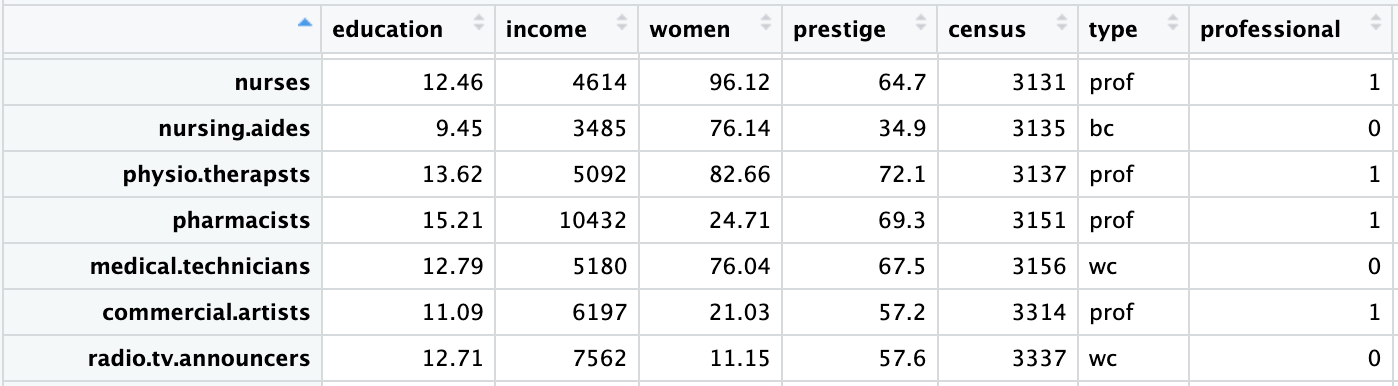
\includegraphics[width=\textwidth]{professionals_column.png}
		\end{figure}
		
	
\newpage
	
	
	\item [(b)]
	Run a linear model with \texttt{prestige} as an outcome and \texttt{income}, \texttt{professional}, and the interaction of the two as predictors (Note: this is a continuous $\times$ dummy interaction.)
		\vspace{.03cm}
		
		In order to run a linear model with a dummy interaction as a predictor, I created an interaction term called \texttt{inter\_1} (\texttt{income} * \texttt{professional}):
			\vspace{.1cm}
	\lstinputlisting[language=R, firstline=27, lastline=27]{PS4.R}  
		\begin{figure}[h!]
			\centering
			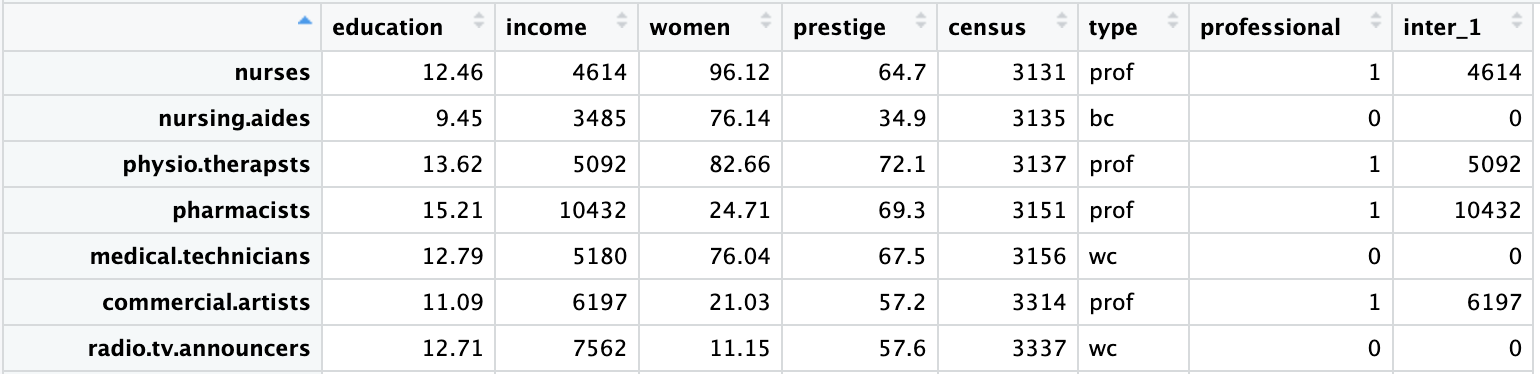
\includegraphics[width=\textwidth]{inter_1_column.png}
		\end{figure}
	
	\vspace{.4cm}
	
		Running the linear model including the interaction term:
	\vspace{.1cm}
	\lstinputlisting[language=R, firstline=30, lastline=31]{PS4.R}  
	
		\begin{verbatim}
	Call:
	lm(formula = prestige ~ income + professional + inter_1, data = Prestige)
	
	Residuals:
	Min      1Q  Median      3Q     Max 
	-14.852  -5.332  -1.272   4.658  29.932 
	
	Coefficients:
	             Estimate   Std. Error  t value  Pr(>|t|)    
	(Intercept)  21.1422589  2.8044261   7.539   2.93e-11 ***
	income        0.0031709  0.0004993   6.351   7.55e-09 ***
	professional 37.7812800  4.2482744   8.893   4.14e-14 ***
	inter_1      -0.0023257  0.0005675  -4.098   8.83e-05 ***
	---
	Signif. codes:  0 ‘***’ 0.001 ‘**’ 0.01 ‘*’ 0.05 ‘.’ 0.1 ‘ ’ 1
	Residual standard error: 8.012 on 94 degrees of freedom
	(4 observations deleted due to missingness)
	Multiple R-squared:  0.7872,	Adjusted R-squared:  0.7804 
	F-statistic: 115.9 on 3 and 94 DF,  p-value: < 2.2e-16
	\end{verbatim}
	
	
	
	\newpage
	
	

	\item [(c)]
	Write the prediction equation based on the result.
		\vspace{.3cm}
	
	\textbf{prestige = 21.142 + 0.003 * income + 37.781 * professional - 0.002 * inter\_1}
	\vspace{.5cm}
	

	\item [(d)]
	Interpret the coefficient for \texttt{income}.
		\vspace{.5cm}
	
		The coefficient for \texttt{income} (0.003) represents the effect of \texttt{income} on \texttt{prestige} when professional is = 0 (blue-collar or white-collar workers).
		For every 1-dollar-unit increase in \texttt{income}, the \texttt{prestige} increases 0.003 for blue-collar or white-collar.
		
		But when \texttt{professional} = 1, the effect of \texttt{income} on \texttt{prestige} changes because of the interaction term coefficient (-0.002 for \texttt{inter\_1}).	In this case, the combined effect of \texttt{income} for \texttt{professionals} is: 0.003 - 0.002 = 0.001.
		
		For 'bc' and 'wc' workers, each additional dollar in income increases prestige by 0.003.
		For professionals, each additional dollar in income increases prestige by 0.001.
	\vspace{1.5cm}
	
	

	\item [(e)]
	Interpret the coefficient for \texttt{professional}.
	\vspace{.2cm}
	
		Being a \texttt{professional} (professional = 1) adds 37.781 points to the \texttt{prestige} score compared to blue-collar or white-collar (professional = 0), when holding \texttt{income} constant.	In another words, when \texttt{income} = 0, \texttt{professionals} have 37.781 points higher \texttt{prestige} than blue-collar or white-collar workers.
	\vspace{1.5cm}
	
	
	
	\item [(f)]
	What is the effect of a \$1,000 increase in income on prestige score for professional occupations? In other words, we are interested in the marginal effect of income when the variable \texttt{professional} takes the value of $1$. Calculate the change in $\hat{y}$ associated with a \$1,000 increase in income based on your answer for (c).
	\vspace{.5cm}

		As we've seeing before in letter (d), for \texttt{professionals} (when professional = 1) each additional 1-unit-dollar in \texttt{income} increases \texttt{prestige} by 0.001 points.  
		
		If we consider \$1,000 dollars increase in \texttt{income}, we have: 1.000 * 0.001 = 1. 
		
		We can conclude that \$1,000 dollars  increase in \texttt{income} is associated with a 1 point increase in the \texttt{prestige} score.
	
	\vspace{.5cm}
	
	\newpage
	
	
	\item [(g)]
	What is the effect of changing one's occupations from non-professional to professional when her income is \$6,000? We are interested in the marginal effect of professional jobs when the variable \texttt{income} takes the value of $6,000$. Calculate the change in $\hat{y}$ based on your answer for (c).
	\vspace{.6cm}
	
	Given the prediction equation for our linear model: 
	
	\textbf{prestige = 21.142 + 0.003 * income + 37.781 * professional - 0.002 * inter\_1}
	\vspace{.4cm}

	
	
	First, we need to calculate $\hat{y}$ for a non-professional (professional = 0). 
	When professional = 0, the interaction term  inter\_1 is also zero:

	\textbf{prestige (non-professional) = 21.142 + 0.003 * 6.000  =  21.142 + 18 = 39.142}
	\vspace{.4cm}

	
	
	Now, we calculate $\hat{y}$ for a professional (professional = 1)
	When professional = 1, we include the interaction term inter\_1:

	\textbf{prestige (professional) = 21.142 + 0.003 * 6.000 + 37.781 - 0.002 *(6.000) = 21.142 + 18 + 37.781 - 12 = 64.923}
	\vspace{.4cm}

	
	
	The marginal effect is the difference between the two prestige scores: 
	
	\textbf{prestige (professional) - prestige (non-professional) = 64.923 - 39.142 = 25.781}
	\vspace{.4cm}


	
	Conclusion: if we change the occupation from a non-professional to a professional when \texttt{income} is \$6.000, it means an increase of 25.781 points in the \texttt{prestige} score.
	

	
\end{enumerate}

\newpage

\section*{Question 2: Political Science}
\vspace{.25cm}
\noindent 	Researchers are interested in learning the effect of all of those yard signs on voting preferences.\footnote{Donald P. Green, Jonathan	S. Krasno, Alexander Coppock, Benjamin D. Farrer,	Brandon Lenoir, Joshua N. Zingher. 2016. ``The effects of lawn signs on vote outcomes: Results from four randomized field experiments.'' Electoral Studies 41: 143-150. } Working with a campaign in Fairfax County, Virginia, 131 precincts were randomly divided into a treatment and control group. In 30 precincts, signs were posted around the precinct that read, ``For Sale: Terry McAuliffe. Don't Sellout Virgina on November 5.'' \\

Below is the result of a regression with two variables and a constant.  The dependent variable is the proportion of the vote that went to McAuliff's opponent Ken Cuccinelli. The first variable indicates whether a precinct was randomly assigned to have the sign against McAuliffe posted. The second variable indicates
a precinct that was adjacent to a precinct in the treatment group (since people in those precincts might be exposed to the signs).  \\

\vspace{.5cm}
\begin{table}[!htbp]
	\centering 
	\textbf{Impact of lawn signs on vote share}\\
	\begin{tabular}{@{\extracolsep{5pt}}lccc} 
		\\[-1.8ex] 
		\hline \\[-1.8ex]
		Precinct assigned lawn signs  (n=30)  & 0.042\\
		& (0.016) \\
		Precinct adjacent to lawn signs (n=76) & 0.042 \\
		&  (0.013) \\
		Constant  & 0.302\\
		& (0.011)
		\\
		\hline \\
	\end{tabular}\\
	\footnotesize{\textit{Notes:} $R^2$=0.094, N=131}
\end{table}

\vspace{.5cm}
\begin{enumerate}
	\item [(a)] Use the results from a linear regression to determine whether having these yard signs in a precinct affects vote share (e.g., conduct a hypothesis test with $\alpha = .05$).
	\vspace{.5cm}
	
	Setting the hypotheses:
	
	\textbf{Null Hypothesis}: Yard signs have no effect on vote share
	
	\textbf{Alternative Hypothesis}: Yard signs affect vote share
	
	\vspace{.3cm}
		
	\lstinputlisting[language=R, firstline=99, lastline=113]{PS4.R}  
	\vspace{.2cm}
	
	Conclusion: As the p-value is $< 0.05$, we can reject the Null Hypothesis and affirm that lawn signs have a significant effect on vote share.
	
	
\vspace{1cm}
	
	
	\item [(b)]  Use the results to determine whether being
	next to precincts with these yard signs affects vote
	share (e.g., conduct a hypothesis test with $\alpha = .05$).
	\vspace{.5cm}
		
	Setting the hypotheses:
	
	\textbf{Null Hypothesis}: being next to precincts with yard signs have no effect on vote share
	
	\textbf{Alternative Hypothesis}: being next to precincts with yard signs affect vote share
	\vspace{.3cm}
	
	\lstinputlisting[language=R, firstline=125, lastline=139]{PS4.R}  
	
	\vspace{.2cm}
		
	Conclusion: As the p-value is $< 0.05$, we can reject the Null Hypothesis. There is sufficient evidence to conclude that being in a precinct adjacent to lawn signs significantly affects vote share at the 5\% significance level.
	
	
\newpage
	
	\item [(c)] Interpret the coefficient for the constant term substantively.
	\vspace{.5cm}
	
		The constant term (intercept) represents the predicted value of the dependent variable when all predictors are set to 0. Considering the regression: 
	
		vote share = 0.302 + 0.042 * assigned signs + 0.042 * adjacent signs, we conclude that the predicted vote share proportion for McAuliff’s opponent, Ken Cuccinelli, in a precinct with no lawn signs (assigned or adjacent) is expected to be 30.2\%.
	
		\vspace{2cm}
	
	

	\item [(d)] Evaluate the model fit for this regression.  What does this	tell us about the importance of yard signs versus other factors that are not modeled?
	\vspace{.5cm}
	
	Considering the data that was given in the 'Impact of lawn signs on vote share' table, we can use the $R^2$ value (0.094) to check if the model fits the regression. The $R^2$ = 0.094 means that only 9.4\% of the variation in vote share is explained by the presence of lawn signs and adjacency to precincts with lawn signs. The remaining 90.6\% (100\% - 9.4\%) of the variation in vote share can be explained by other factors not included in the model, such as campaign strategies, demographics issues, etc.
	
	Even though lawn signs and adjacency significantly affect vote share as we saw before, their overall impact is small and they are not a major factor in determining vote share.
	
	
	
\end{enumerate}  


\end{document}
